\documentclass[a4paper,oneside]{article}

\usepackage{graphicx}
% \usepackage{url}
\usepackage{hyperref}
\usepackage{fancyhdr} 
\pagestyle{fancy}


\usepackage{listings}
\usepackage{courier}
\lstset{
         basicstyle=\footnotesize\ttfamily, % Standardschrift
         %numbers=left,               % Ort der Zeilennummern
         numberstyle=\tiny,          % Stil der Zeilennummern
         %stepnumber=2,               % Abstand zwischen den Zeilennummern
         numbersep=5pt,              % Abstand der Nummern zum Text
         tabsize=2,                  % Groesse von Tabs
         extendedchars=true,         %
         breaklines=true,            % Zeilen werden Umgebrochen
         keywordstyle=\color{red},
    		frame=b,         
 %        keywordstyle=[1]\textbf,    % Stil der Keywords
 %        keywordstyle=[2]\textbf,    %
 %        keywordstyle=[3]\textbf,    %
 %        keywordstyle=[4]\textbf,   \sqrt{\sqrt{}} %
         stringstyle=\color{white}\ttfamily, % Farbe der String
         showspaces=false,           % Leerzeichen anzeigen ?
         showtabs=false,             % Tabs anzeigen ?
         xleftmargin=17pt,
         framexleftmargin=17pt,
         framexrightmargin=5pt,
         framexbottommargin=4pt,
         %backgroundcolor=\color{lightgray},
         showstringspaces=false      % Leerzeichen in Strings anzeigen ?        
}
\lstloadlanguages{C}
% Check Dokumentation for further languages ...
         %[Visual]Basic
         %Pascal
%          C
         %C++
         %XML
         %HTML
         %Java
% }
%\DeclareCaptionFont{blue}{\color{blue}} 

%\captionsetup[lstlisting]{singlelinecheck=false, labelfont={blue}, textfont={blue}}
\usepackage{caption}
\DeclareCaptionFont{white}{\color{white}}
\DeclareCaptionFormat{listing}{\colorbox[cmyk]{0.43, 0.35, 0.35,0.01}{\parbox{\textwidth}{\hspace{15pt}#1#2#3}}}
\captionsetup[lstlisting]{format=listing,labelfont=white,textfont=white, singlelinecheck=false, margin=0pt, font={bf,footnotesize}}



\bibliographystyle{unsrt} 
\newenvironment{mylisting}
{\begin{list}{}{\setlength{\leftmargin}{1em}}\item\scriptsize\bfseries}
{\end{list}}
\newenvironment{mytinylisting}
{\begin{list}{}{\setlength{\leftmargin}{1em}}\item\tiny\bfseries}
{\end{list}}


\title{Tutorial:\\Rare Event Sampling with FRESHS and FFS\\using the example of a\\1D particle in a double well potential.}
\author{Kai Kratzer}


\begin{document}
\lhead{Rare Event Sampling with FRESHS}
\rhead{
\includegraphics[height=0.06\linewidth]{../espresso-ffs/pics/freshs-logo.png}}
% \lfoot{Kratzer, Berryman, Arnold}

\maketitle
\tableofcontents

\newpage

\section{Simulation problem}

In this tutorial we perform FFS simulations of a 1D particle in a double well potential using FRESHS~\cite{freshs}. For the simulations, we use a velocity verlet integrator and a Langevin thermostat, set up in a custom python harness script.
\begin{figure}
 \centering
 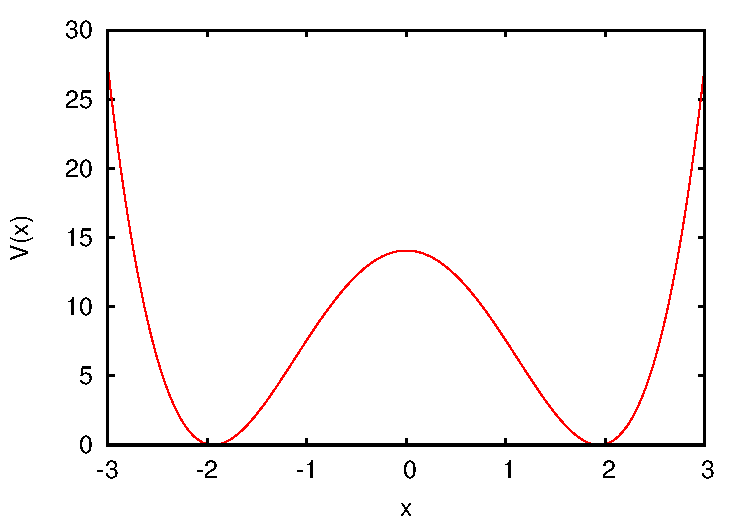
\includegraphics[width=0.9\linewidth]{fig/potential}
 \caption{Double well potential.}
 \label{fig:dw}
\end{figure}
The potential (see also fig.~\ref{fig:dw}) from which the forces are derived is given by
\begin{equation}
 V(x)=x^4-7.5x^2+14.0625.
\end{equation}
The particle is set up at the left-hand side of the barrier with $x<-1.5$. We are interested in pushing the particle over the barrier using FFS. Therefore, we set $\lambda_A=-1.5$ and $\lambda_B=1.5$. We use the automatic optimized interface placement~\cite{optiflux} with exploring scouts and a target probability of $p=0.5$ to set up the scenario automatically. All values are pre-defined in the configuration scripts, but feel free to play around.


\section{Getting started}

\begin{enumerate}
 \item Clone the latest FRESHS code from github:
\begin{mylisting}
\begin{verbatim}
git clone https://github.com/freshs/freshs.git
\end{verbatim}
\end{mylisting}
 \item Navigate to 
\begin{mylisting}
\begin{verbatim}
freshs/server
 \end{verbatim}
\end{mylisting}
 \item Have a look at the configuration file
\begin{mylisting}
 \begin{verbatim}
  server-python-ffs_tutorial.conf
 \end{verbatim}
\end{mylisting}
 and make changes if desired.
 \item Start the server for this tutorial with
\begin{mylisting}
\begin{verbatim}
python main_server.py -c server-python-ffs_tutorial.conf
\end{verbatim}
\end{mylisting}
 \item Open a second terminal and navigate to
\begin{mylisting}
\begin{verbatim}
freshs/harnesses/python-ffs_tutorial
\end{verbatim}
\end{mylisting}
Open the job\_script and look if the physics is calculated correctly. Then, navigate to
\begin{mylisting}
\begin{verbatim}
freshs/client
\end{verbatim}
\end{mylisting}
 \item Start the client with
\begin{mylisting}
\begin{verbatim}
python main_client.py -c client-python-ffs.conf
\end{verbatim}
\end{mylisting}
\end{enumerate}
The client starts the harness script specified in its configuration file which then performs the calculation of the physics.

Wait for the simulation to finish. If you can't wait, download a ready populated database for this example\footnote{\url{http://www.freshs.org/dw/lib/exe/fetch.php?media=tutorial:2014-04-22_19-24-53_configpoints.sqlite.gz}}. Note that for this small example we have a lot of communication overhead, because the runs are very short. In a `real' simulation the computation time should take the largest amount of time.


\section{Postprocessing}

\subsection{Database view}
If you have the `sqlitebrowser' or the firefox `SQLite Manager' plugin installed, then you could use them to have a look at the raw data which comprises the output database, which contains the state at the end of the fragment, as well as enough information to re-generate it (i.e.~a pointer to the parent fragment, and an RNG seed).
You can also use the commandline tool `sqlite3' to manipulate the database directly, but don't forget to do a backup first!

The database can be already analyzed and viewed during the simulation. Note, that you should not write to the database during the simulation, handle with care. If the simulation fails at a certain stage, data can be modified/deleted, and the simulation can be resumed from the last state in the database using the `-r' flag of the server.

\subsection{Analysis scripts}
The folder `scripts' in your FRESHS directory contains analysis scripts which can be used directly to e.g. backtrack successful runs or to serve as templates for own analysis scripts.

\subsubsection{Backtracking successful runs}
Change to the `freshs/scripts' folder and run the following script:
\begin{mylisting}
\begin{verbatim}
python ffs_python-tutorial-analysis.py /tmp/DB/<timestamp>_configpoints.sqlite
\end{verbatim}
\end{mylisting}
The output is written to a folder called `OUTPUT/timestamp'. Change to this directory, start gnuplot and plot the tree graph to visualize the traces which lead to the points on the last known interface:
\begin{mylisting}
\begin{verbatim}
load "tree_success.gnuplot"
\end{verbatim}
\end{mylisting}
If you'd like to plot the pathways and configuration points, you could do it like this:
\begin{mylisting}
\begin{verbatim}
plot "trace0.dat" u 1:4 w p, "trace0.path" w l
\end{verbatim}
\end{mylisting}


\subsubsection{Interface statistics}
To plot statistical information about the simulation, e.g. a histogram of the runtime of the clients or a histogram of the calculation steps, run
\begin{mylisting}
\begin{verbatim}
./ffs_interfaces_statistics.py /tmp/DB/<timestamp>_configpoints.sqlite
\end{verbatim}
\end{mylisting}
The output is written again to the folder called `OUTPUT/timestamp'. Change to this directory, start gnuplot and plot the histograms:
\begin{mylisting}
\begin{verbatim}
load "histo_runtime.gnuplot"
load "histo_calcsteps.gnuplot"
\end{verbatim}
\end{mylisting}


\subsubsection{Energy landscape}
The energy landscape can be extracted from the distribution of the order parameter during the simulation and by weighting with the particular transition probabilities~\cite{stadist}:
\begin{mylisting}
\begin{verbatim}
python ffs_python-tutorial-energy-profile.py /tmp/DB/<timestamp>_configpoints.sqlite
\end{verbatim}
\end{mylisting}
The output is written again to the folder called `OUTPUT/timestamp'. Change to this directory, start gnuplot and plot the energy landscape and the potential:
\begin{mylisting}
\begin{verbatim}
V(x)=(x**4.0)-7.5*(x**2)+14.0625+c
fit V(x) "data_dG.dat" via c
plot "data_dG.dat", V(x)
\end{verbatim}
\end{mylisting}


\begin{thebibliography}{1}

\bibitem{freshs}
K.~Kratzer, J.~T. Berryman, A.~Taudt, and A.~Arnold.
\newblock {The Flexible Rare Event Sampling Harness System (FRESHS)}.
\newblock {\em Comp. Phys. Comm.}, 2014.

\bibitem{optiflux}
K.~Kratzer, A.~Arnold, and R.~J. Allen.
\newblock Automatic, optimized interface placement in forward flux sampling
  simulations.
\newblock {\em J. Chem. Phys.}, 138(16):164112, 2013.

\bibitem{stadist}
C.~Valeriani, R.J.~Allen, M.J.~Morelli, D.~Frenkel, and P.R.~ten~Wolde.
\newblock Computing stationary distributions in equilibrium and nonequilibrium systems with forward flux sampling.
\newblock {\em J. Chem. Phys.}, 127, 114109, 2007.

\end{thebibliography}


\end{document}
